\documentclass{beamer}
\usepackage{amsfonts,amsmath,oldgerm}
\usepackage{ragged2e}

\usetheme{sintef}

\newcommand{\testcolor}[1]{\colorbox{#1}{\textcolor{#1}{test}}~\texttt{#1}}

\usefonttheme[onlymath]{serif}

\titlebackground*{assets/background}

\newcommand{\hrefcol}[2]{\textcolor{cyan}{\href{#1}{#2}}}

\title{Aula Zero - Programa da Disciplina}
\subtitle{2023.1 - LESA 6 -  Laboratório de Escalabilidade de Sistemas}
\course{Tecnologia em Análise e Desenvolvimento de Sistemas}
\author{\href{mailto:luiz.quirino@ifsp.edu.br}{Luiz \textbf{Quirino}}}
\IDnumber{luiz.quirino@ifsp.edu.br}



\begin{document}
\maketitle

%\begin{frame}
%
%      Este material é produzido utilizando \LaTeX\, baseado na SINTEF Presentation, disponibilizado sob licenciamento \hrefcol{https://creativecommons.org/licenses/by-nc/4.0/legalcode}{Creative Commons CC BY 4.0}
%
%\vspace{\baselineskip}

%In the following you find a brief introduction on how to use \LaTeX\ and the beamer package to prepare slides, based on the one written by \hrefcol{mailto:federico.zenith@sintef.no}{Federico Zenith} for \hrefcol{https://www.overleaf.com/latex/templates/sintef-presentation/jhbhdffczpnx}{SINTEF Presentation}

% This template is released under \hrefcol{https://creativecommons.org/licenses/by-nc/4.0/legalcode}{Creative Commons CC BY 4.0} license
%\end{frame}
\footlinecolor{sintefdarkgreen}
\section{Apresentação docente}

\begin{frame}{Sobre o docente:}
Formação:
\begin{itemize}
\item Pós-graduação em Gestão de Riscos e CiberSegurança - Faculdade Focus
\item Sistemas de Informação - UFMS
\item Gestão de Tecnologia da Informação - Unicesumar
\item Técnico em Informática - Centro Paula Souza
\end{itemize}
Áreas de Interesse:
\begin{itemize}
\item Gestão de Tecnologia da Informação
\item Governança de Tecnologia da Informação
\item Gestão de Riscos e CiberSegurança
\item Desenvolvimento de software
\end{itemize}
\end{frame}

\section{Apresentação da disciplina}

\begin{frame}{Ementa}\justifying
      O componente curricular apresenta e discute os conceitos teóricos, as aplicações práticas
de ferramentas e os impactos que os requisitos de escalabilidade trazem para definição da
arquitetura de um sistema.
\end{frame}

\begin{frame}{Objetivo da disciplina}\justifying
      Compreender os tipos de escalabilidade de sistemas: vertical e horizontal\newline
      \newline
      Aplicar técnicas e
      ferramentas para escalabilidade de serviços web.\newline
      \newline
      Identificar e implementar estratégias de cache em diferentes níveis do sistema
\end{frame}

\begin{frame}{Objetivo da disciplina}\justifying
      Utilizar mecanismos de processamento assíncrono
      como filas de mensagem e identificar cenários de uso para arquitetura orientada a eventos \newline
      \newline
      Compreender e implementar soluções para escalabilidade de dados como técnicas de
replicação, particionamento, aplicação de bancos NoSQL e utilização de sistemas para
busca e análise de grandes volumes de dados.\newline
      \newline
      Realizar e avaliar resultados de testes de
      desempenho, de carga e de estresse.
      
\end{frame}

\begin{frame}{Conteúdo Programático}\justifying
      \begin{itemize}
            \item Escalabilidade de Sistemas
                  \begin{itemize}
                        \item Escalabilidade Vertical e Horizontal
                        \item Visão Geral da Infraestrutura de um Data Center
                  \end{itemize}
            
            
      \end{itemize}
\end{frame}

\begin{frame}{Conteúdo Programático}\justifying
      \begin{itemize}
            \item Escalabilidade de Serviços Web
            \begin{itemize}
                  \item Arquitetura Monolítica vs Microserviços
                  \item Arquitetura Stateless vs. Statefull
                  \item Function as a Service (FaaS) e Serverless Computing (Backend as a Service)
                  \item Balanceamento de Carga (Load Balance)
                  \item Afinidade de Sessão (Sticky Session), Replicação de Sessão e Armazenamento de Sessão Centralizado (Centralized Session Storage)
                  \item Estratégias de Autenticação e Autorização 
            \end{itemize}
           
      \end{itemize}
\end{frame}
\begin{frame}{Conteúdo Programático}\justifying
      \begin{itemize}
            \item Estratégias de Caching
            \begin{itemize}
                  \item HTTP Cache 
                  \item Proxy Reverso
                  \item Content Delivery Networks (CDN) 
                  \item Cache de Objetos
                  \item Cache Distribuído
            \end{itemize}
           
      \end{itemize}
\end{frame}
\begin{frame}{Conteúdo Programático}\justifying
      \begin{itemize}
            \item Processamento Assíncrono
            \begin{itemize}
                  \item Fila de Mensagens (Message Queue)
                  \item Arquitetura Orientada a Eventos
            \end{itemize}
           
      \end{itemize}
\end{frame}

\begin{frame}{Conteúdo Programático}\justifying
      \begin{itemize}
            \item Escalabilidade de Dados
            \begin{itemize}
                  \item Replicação (Replication)
                  \item Particionamento (Sharding) 
                  \item Escalabilidade com NoSQL
                  \item Busca e Análise de Grandes Volumes de Dados 
            \end{itemize}
           
      \end{itemize}
\end{frame}
\begin{frame}{Conteúdo Programático}\justifying
      \begin{itemize}
            \item Teste de Desempenho
            \begin{itemize}
                  \item Levantamento de Cenários
                  \item Teste de Desempenho
                  \item Teste de Carga
                  \item Teste de Estresse
                  \item Identificação de Gargalos
            \end{itemize}
           
      \end{itemize}
\end{frame}

\begin{frame}{Bibliografia básica}\justifying
      \begin{itemize}
            \item \textbf{BRITO, Samuel Henrique Bucke. \textcolor{sintefdarkgreen}{Serviços de rede em servidores Linux. 1. ed.}} São Paulo: Novatec, 2017. ISBN 9788575226193.
            \item \textbf{ SADALAGE, Pramod J.; FOWLER, Martin. \textcolor{sintefdarkgreen}{NoSQL essencial: um guia conciso para o mundo emergente da persistência poliglota. 1. ed.}} São Paulo: Novatec, 2013. ISBN 9788575223383.
            \item \textbf{ VERAS, Manoel. \textcolor{sintefdarkgreen}{Computação em nuvem: nova arquitetura de TI. 1. ed.}} Rio de Janeiro: Brasport, 2015. ISBN 9788574527529. Disponível em: https://ifsp.bv3.digitalpages.com.br/users/publications/9788574527529. Acesso em: 14 jun. 2019.     
      \end{itemize}
\end{frame}
      

\begin{frame}{Bibliografia complementar}
      \begin{itemize}
            \item \textbf{DATE, C. J. \textcolor{sintefdarkgreen}{Introdução aos sistemas de bancos de dados.}} Rio de Janeiro: Campus, 2004. ISBN 9788535212730.
            \item \textbf{ELMASRI, Ramez; NAVATHE, Shamkant B. \textcolor{sintefdarkgreen}{Sistemas de banco de dados. 7. ed.}} São Paulo: Pearson Addison Wesley, 2018. ISBN 9788543025001. Disponível em: https://ifsp.bv3.digitalpages.com.br/users/publications/9788543025001. Acesso em: 14 jun. 2019.
            \item \textbf{OLONCA, Ricardo Lino. \textcolor{sintefdarkgreen}{Administração de redes Linux. 1. ed.}} São Paulo: Novatec, 2015. ISBN 9788575224618. 
           
      \end{itemize}
\end{frame}

\begin{frame}{Bibliografia complementar}
      \begin{itemize}
            \item \textbf{SHOTTS JR, William E. \textcolor{sintefdarkgreen}{The linux command line: a complete introduction. 5. ed.}} San Francisco: No Starch Press, 2019. Disponível em: http://linuxcommand.org/tlcl.php. Acesso em: 14 jun. 2019.
            \item \textbf{SOMMERVILLE, Ian. \textcolor{sintefdarkgreen}{Engenharia de software. 9. ed.}} São Paulo: Pearson Prentice Hall, 2011. ISBN 9788579361081. Disponível em: https://ifsp.bv3.digitalpages.com.br/users/publications/9788579361081. Acesso em: 14 jun. 2019.
            
      \end{itemize}
\end{frame}

\section{Planejamento}


\begin{frame}[fragile]{Planejamento de aulas}
      \begin{columns}
            \begin{column}{0.5\textwidth}
                  \textbf{Definições da disciplina:}
                  \begin{itemize}
                        \item Total de aulas: 38 
                        \item Aulas semanais: 2 (19 semanas)
                        \item Total de horas: 28,50
                        \item Atividades práticas (divididas em entregas mensais, a partir de setembro)
                        \item Atividades teoricas (discussões em sala)
                        \item Desenvolvimento de projeto final
      
                  \end{itemize}


            \end{column}
            \begin{column}{0.5\textwidth}
                  \textbf{Turma: 324025}
                  \begin{itemize}
                        \item Sextas-feiras: 21:20 - 22:50
                        \item Período: 28/07 - 01/12 (08/12 - IFA)
                        \item Feriados: 08/09 - 13/10 - 03/11
                        \item Eventos: 22/09
                  \end{itemize}
                  
            \end{column}
      \end{columns}
\end{frame}



%\section{Moodle}

%\begin{frame}[fragile]{Auto Inscrição Moodle}
%
%      \textbf{Autoinscrição → \textcolor{sintefred}{Chave: IFSP@2023.2}}
%
%      \begin{figure}[H]
%            \centerline{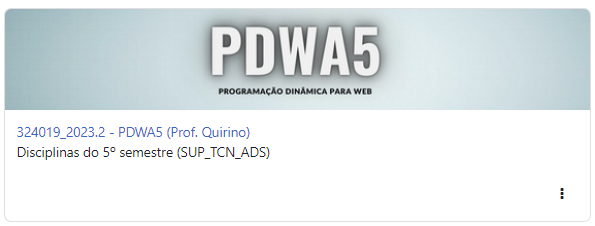
\includegraphics[width=1\textwidth]{assets/aula-tads-pdwa5/moodle_quinta.png}}
%            
%        \end{figure}
%        
%\end{frame}


\section{Avaliações}

\begin{frame}[fragile]\justifying
\frametitle{Sistema de avaliação}
\begin{itemize}
            
            \item Como seremos avaliados:
            \begin{itemize}
                  \item Um trabalho teórico(TT) que atenderá 30\% da nota;
                  \item Um trabalho prático(TP) que atenderá 30\% da nota;
                  \item Atividades avaliativas/participação em aula (AA), contando como 30\% da nota;
            \end{itemize}
            \item Em caso de não obtenção dos critérios mínimos para aprovação, aplicação de IFA por meio de prova teórica, escrita, presencial;
\end{itemize}
\begin{colorblock}[black]{sinteflightgreen}{ATENÇÃO}
      Os trabalhos serão disponibilizados a \textbf{partir da 5ª aula ministrada} na disciplina, contando com documentação disponibilizado pelo docente, ficando aberta para entregas sucessivas no moodle.
      Os trabalhos teórico e prático são interdepentes, sendo a parte teórica / descritiva fudamentada na implementação da atividade prática;
\end{colorblock}

\end{frame}

\begin{frame}[fragile]\justifying
      \frametitle{Sistema de avaliação}
      \begin{itemize}
            \item Média trabalho \[ MT = TP * 0,45 + TT * 0,25\]
            \item Média produtividade \[ MP = \left ( \frac{AA_1 + AA_2 + ... + AA_n}n \right ) * 0,3 \]
            \item Média Final - MF \[MF = MT + MP\]
      \end{itemize}
      
      \end{frame}


\begin{frame}[fragile]\justifying
      \frametitle{Critérios de avaliação}
      Respeitando ao disposto no PPC vigente do curso, no item \textbf{\textit{8. AVALIAÇÃO DA APRENDIZAGEM. }}
      \newline
      \newline
      \textit{Os critérios de aprovação nos componentes curriculares, envolvendo simultaneamente frequência e avaliação, para os cursos da Educação Superior de 
      regime semestral, são a obtenção, no componente curricular, de nota semestral igual ou superior a 6,0 (seis) e frequência mínima de 75\% (setenta e cinco por cento) das
      aulas e demais atividades. }
\end{frame}

\begin{frame}[fragile]\justifying
      \frametitle{Critérios de avaliação}
      \textit{Fica sujeito ao Instrumento Final de Avaliação (IFA), o estudante que obtenha, no componente curricular, nota semestral igual ou superior a
      4,0 (quatro) e inferior a 6,0 (seis) e frequência mínima de 75\% (setenta e cinco por cento) das aulas e demais atividades. O estudante que realizar o Instrumento Final de
      Avaliação, para ser aprovado, deverá obter a nota mínima igual a 6,0 (seis). A nota final considerada, para registros escolares, será a maior entre a nota semestral e a nota do
      Instrumento Final de Avaliação (IFA). 
      \newline
      \newline
      É importante ressaltar que os critérios de avaliação na Educação Superior primam pela autonomia intelectual.}
\end{frame}

\section{Conduta ética}
\begin{frame}
\frametitle{Termos de Conduta}
      \begin{itemize}
            \item Trabalhos e provas devem ser feitas INDIVIDUALMENTE;
            \item Cada estudante tem responsabilidade sobre cópias de suas implementações e provas, mesmo que parciais;
            \item Não faça implementeções em grupo e não compartilhe programas ou trechos de programas;
            \item Você pode consultar seus colegas para esclarecer dúvidas e discutir idéias sobre implementações, mas NÃO copie programas!
            \item Implementações e provas consideradas plagiadas terão nota ZERO;
            \item O estudante que se envolver em DOIS CASOS DE PLÁGIO estará automaticamente REPROVADO na disciplina.
      \end{itemize}
\end{frame}

\section{Informações sobre os slides}

\footlinecolor{sintefyellow}
\begin{frame}[fragile]{Dicas sobre os slides}
      
      \begin{itemize}
            \item Slides com rodapé em vermelho foram adicionados após a aula dada;
            \item Slides com rodapé em amarelo foram atualizados  após a aula dada.
      \end{itemize}
\end{frame}

\footlinecolor{sintefred}
\begin{frame}[fragile]{Imagem do dia}

        \begin{figure}[H]
            \centerline{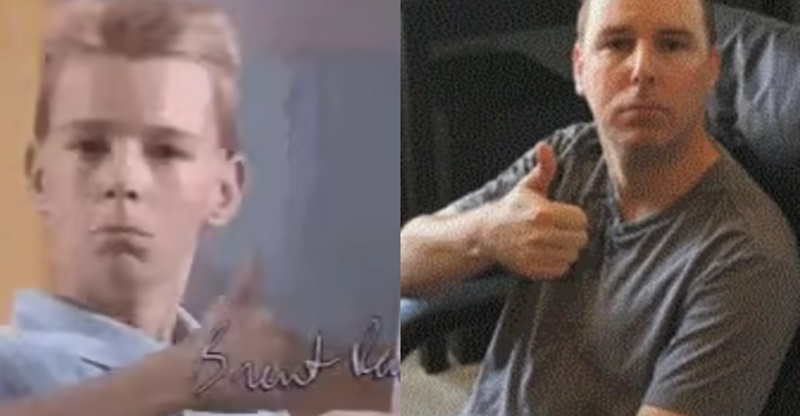
\includegraphics[width=0.8\textwidth]{assets/imagem-do-dia/brent_rambo.jpg}}
            
        \end{figure}
\end{frame}


\footlinecolor{}

\backmatter
\end{document}
